\documentclass[12pt]{article}
\setlength{\oddsidemargin}{0in}
\setlength{\evensidemargin}{0in}
\setlength{\textwidth}{6.5in}
\setlength{\parindent}{0in}
\setlength{\parskip}{\baselineskip}
\usepackage{amsmath,amsfonts,amssymb}
\usepackage{graphicx}
\usepackage[]{algorithmicx}
\usepackage{enumitem}
\usepackage{fancyvrb}

\usepackage{fancyhdr}
\pagestyle{fancy}
\setlength{\headsep}{36pt}

\usepackage{hyperref}
\graphicspath{{F:/Users/sasha/Documents/Summer 2020/Algo/Midterm}}

\hypersetup{
    colorlinks=true,
    linkcolor=blue,
    filecolor=magenta,      
    urlcolor=blue,
}

\newcommand{\makenonemptybox}[2]{%
%\par\nobreak\vspace{\ht\strutbox}\noindent
\item[]
\fbox{% added -2\fboxrule to specified width to avoid overfull hboxes
% and removed the -2\fboxsep from height specification (image not updated)
% because in MWE 2cm is should be height of contents excluding sep and frame
\parbox[c][#1][t]{\dimexpr\linewidth-2\fboxsep-2\fboxrule}{
  \hrule width \hsize height 0pt
  #2
 }%
}%
\par\vspace{\ht\strutbox}
}
\makeatother

\begin{document}
\lhead{{\bf CSCI 3104, Algorithms \\ Mid Term exam Summer 2020 (30 points)  } }
\rhead{Name: \fbox{Sasha Farhat % Place your name here and delete the next time
\phantom{This is a really long name}} 
\\ ID: \fbox{105887541 %+ Place your ID here and delete the next time
\phantom{This is a student ID}} 
\\ {\bf Escobedo \& Jahagirdar\\ Summer 2020, CU-Boulder}}
\renewcommand{\headrulewidth}{0.5pt}

\phantom{Test}

\begin{small}
\textit{Advice 1}:\ For every problem in this class, you must justify your answer:\ show how you arrived at it and why it is correct. If there are assumptions you need to make along the way, state those clearly.
%\vspace{-3mm} 

\textit{Advice 2}:\ Verbal reasoning is typically insufficient for full credit. Instead, write a logical argument, in the style of a mathematical proof.\\
%\vspace{-3mm} 

\textbf{Honor code}: On my honor as a University of Colorado at Boulder student,
I have neither given nor sought unauthorized assistance in this work\\  \\
\textbf{Initials} 
\fbox{S.F.% Place your iniitals here and delete the next time
\phantom{This is a really long name}} \\ \\
\textbf{Date} 
\fbox{06/27/2020 % Place your Date here and delete the next time
\phantom{This is a really long name}} \\ 


If you violate the CU \textbf{Honor Code}, you will receive a 0.

\textbf{Instructions for submitting your solution}:
\vspace{-5mm} 

\begin{itemize}
	\item The solutions \textbf{should be typed}, we cannot accept hand-written solutions. Here's a short intro to \href{http://ece.uprm.edu/~caceros/latex/introduction.pdf}{\textbf{Latex}.}
	 \item In this homework we denote the asymptomatic \textit{Big-O} notation by $\mathcal{O}$ and \textit{Small-O} notation is represented as $o$. 
	\item We recommend using online Latex editor \href{https://www.overleaf.com/}{\textbf{Overleaf}}. Download the \textbf{.tex} file from Canvas and upload it on overleaf to edit.
	%todo add link of gradescope
	\item You should submit your work through \href{https://www.gradescope.com}{\textbf{Gradescope}}  only.
	\item If you don't have an account on it, sign up for one using your CU email. You should have gotten an email to sign up. If your name based CU email doesn't work, try the identikey@colorado.edu version. 
	\item Gradescope will only accept \textbf{.pdf} files (except for code files that should be submitted separately on Canvas if a problem set has them) and \textbf{try to fit your work in the box provided}. 
	\item You cannot submit a pdf which has less pages than what we provided you as Gradescope won't allow it.
   
\end{itemize}
\vspace{-4mm} 
\end{small}

%\hrulefill



\textbf{Master Method}: Consider a recurrence relation of the form \\
\begin{equation*}
    T(n)  = aT(n/b) + f(n)
\end{equation*}
where $a \ge 1$ and $b > 1$ are constants, and $T(n) = constant$ for $n \le 1$. \\
The asymptotic growth of T(n) is bounded as follows: 
\begin{itemize}
    \item \textbf{Case 1} $f(n) = \mathcal{O}(n^{\log_ba - \epsilon})$ for some constant $\epsilon>0$ $\implies$ $T(n) = \Theta(n^{\log_ba})$
    \item \textbf{Case 2} $f(n) = \Theta(n^{\log_ba})$  $\implies$ $T(n) = \Theta(n^{\log_ba} \log(n))$
    \item \textbf{Case 3} $f(n) = \Omega(n^{\log_ba +\epsilon})$ for some constant $\epsilon>0$ and if $af(\frac{n}{b}) \le c f(n)$ for some constant $c<1$ and all sufficiently large $n$. $\implies$ $T(n) = \Theta(f(n))$
\end{itemize}

\textbf{Formulae} 
\begin{itemize}
    \item $1+2+3+....+n = \frac{n(n+1)}{2}$
    \item $1^2+2^2+.....+n^2 = \frac{n(n+1)(2n+1)}{6}$ 
    \item \textbf{Sequences} The formulae for the sum of an Arithmetic Progression (AP) and Geometric Progression (GP) are available  \href{https://www.a-levelmaths.com/Summary%20Handouts/Arithmetic%20and%20Geometric%20Progressions%20APGP%20Summary.pdf}{here}
\end{itemize}

\pagebreak

\begin{enumerate}

	\item{ (3 pts) 
	Which of $\mathcal{O}$, $\Omega$ or $\Theta$ is the correct asymptotic relationship for $f(n) = n^{\frac{1}{3}} \log_3(n)$ compared
    to $g(n) = \sqrt{n}$? Write your answer as $f(n) = \tau(g)$ where $\tau$  should be replaced by
    the appropriate symbol ($\mathcal{O}, \Omega, \Theta$), show the necessary work to justify your answer.}
    \makenonemptybox{6in}{
    $f(n)=n^{\frac{1}{3}}\log_3(n)$\\
    $g(n)= \sqrt{n}$\\
    $f(n)= \Omega(g(n))$\\
    \\
    $0 \leq c\cdot g(n) \leq f(n)$\\
    \\
    $0\leq c \cdot n^{\frac{1}{2}}\leq n^{\frac{1}{3}}\log_3n$\\
    \\
    $0 \leq c\cdot n^{\frac{1}{6}} \leq \log_3n $\\
    \\
    Setting arbitrary value for $n_0$ we can prove that there is a constant $c$ where the ineualities hold true.\\
    $n_0 = 3^6$\\
    $0 \leq c \cdot \sqrt[6]{3^6} \leq log_3 (3^6)$\\
    $0 \leq c \cdot 3 \leq 6$\\
    $c = 1$\\
    Since there is a value $n_0$ and $c$ that make the statement true: \textbf{$f(n)=\Omega(g(n))$}
    }
	\clearpage
	\item{ (2 pts) 
	Which of $\mathcal{O}$, $\Omega$ or $\Theta$ is the correct asymptotic relationship for $f(n) = \frac{n^2 - 8n + 15}{n-5}$ compared
    to $g(n) = \frac{1^2+2^2+....+ n^2}{1+2+...+n}$? Write your answer as $f(n) = \tau(g)$ where $\tau$  should be replaced by
    the appropriate symbol ($\mathcal{O}, \Omega, \Theta$), show the necessary work to justify your answer}
    \makenonemptybox{6.2in}{
    $f(n) = \frac{n^2 - 8n + 15}{n-5}$\\
    $g(n) = \frac{1^2+2^2+....+ n^2}{1+2+...+n}$\\
    \\
    $f(n)=\Theta(g(n))$\\
    $0\leq c_1 \cdot g(n)\leq f(n)\leq c_2 \cdot g(n)$\\
    \\
    $0\leq c_1 \cdot \frac{1^2+2^2+....+ n^2}{1+2+...+n}\leq \frac{n^2 - 8n + 15}{n-5}\leq c_2 \cdot \frac{1^2+2^2+....+ n^2}{1+2+...+n}$\\
    \\
    Both f(n) abd g(n) have arbitrary constants added to their equations. By keeping the largest variable and removing the added constants without changing f(n) and g(n) graph trend, we can evaluate the inequalities easier.
    \\
    $0\leq c_1 \cdot \frac{n^2}{n}\leq \frac{n^2 }{n}\leq c_2 \cdot \frac{n^2}{n}$\\
    \\
    $0\leq c_1 \cdot n\leq n\leq c_2 \cdot n$\\
    We can clearly see that f(n) is tightly bound by g(n) for there is a constant c such that $0\leq c_1 \cdot g(n)\leq f(n)\leq c_2 \cdot g(n)$ holds true. Therefore $f(n)=\Theta(g(n))$
	}
	\item{ (1 pts)
	State True or false without justification\\
	If the running time of an algorithm satisfies the recurrence relation \\
    $T(n) = T(n/18) + T(17n/18) + cn$, 
    then $T(n) = \mathcal{O}(n\log(n))$.
    }
    \makenonemptybox{0.5in}{
    True
    }

    \item{ (1 pts)
    Let $H$ be a hash table with 2020 slots with a hash function $h(x)$ that satisfies \textbf{uniform hashing} property. Given two items $x_1$, $x_2$, what is the probability that they do not hash to the same location?
    }
    \makenonemptybox{3in}{
    The probability that the two items hash into the same location is $\frac{1}{m}$, where m is the table size. The probability that they do not hash to the same location is $1-\frac{1}{m}=\frac{2019}{2020}$.
    }
    \clearpage
    \item{ (3 pts) 
    Suppose $T(n) = T(n - 5) + n$, where $T(n) = \Theta(1)$ if $ n \le 5$.  Find a function $g(n)$ such that $T(n) = \Theta(g(n))$. Clearly justify your answer.
    }
    \makenonemptybox{6in}{
    Given:
    $T(n) = T(n - 5) + n$ $\rightarrow$ $n>5$, and $=1$ $\rightarrow$ $n\leq 5$ \\
    \\
    $T(n)= T(n-5)+n$\\
    $=T(n-10)+(n-5)+n$\\
    $=T(n-15)+(n-10)+(n-5)+n$\\
    $=T(n-20)+(n-15)+(n-10)+(n-5)+n$\\
    .\\
    .\\
    .\\
    $T(1)+ ...+ (n-10)+(n-5)+n$\\
    \\
    we see that we have $\frac{n}{5}$ terms\\
    We get the equeation $T(n)=T(1)+(\frac{n}{5})(n)$\\
    $=1+n\cdot\frac{n}{5}$\\
    \\
    ignoroing the constants we get $g(n)= n^2$ such that $T(n)=\Theta(g(n))$
    }
    \clearpage
    \item{ (1 pt)
    For the set $\Sigma = \{ a, b, c\}$, give the set of inequalities on the frequencies $f_a, f_b, f_c$ that would yield the corresponding codewords ${00, 01, 1}$ respectively under Huffman's algorithm.  Assume that while constructing the tree, we merge  two nodes such that the node with least frequency is the left child. In your tree branching left corresponds to 0 and branching right corresponds to 1. List the frequencies $f_a, f_b, f_c$ below that produce the specified codewords.  Your choice of frequencies should \textbf{always} produce the same tree/codes provided.
    }
    \makenonemptybox{2in}{
    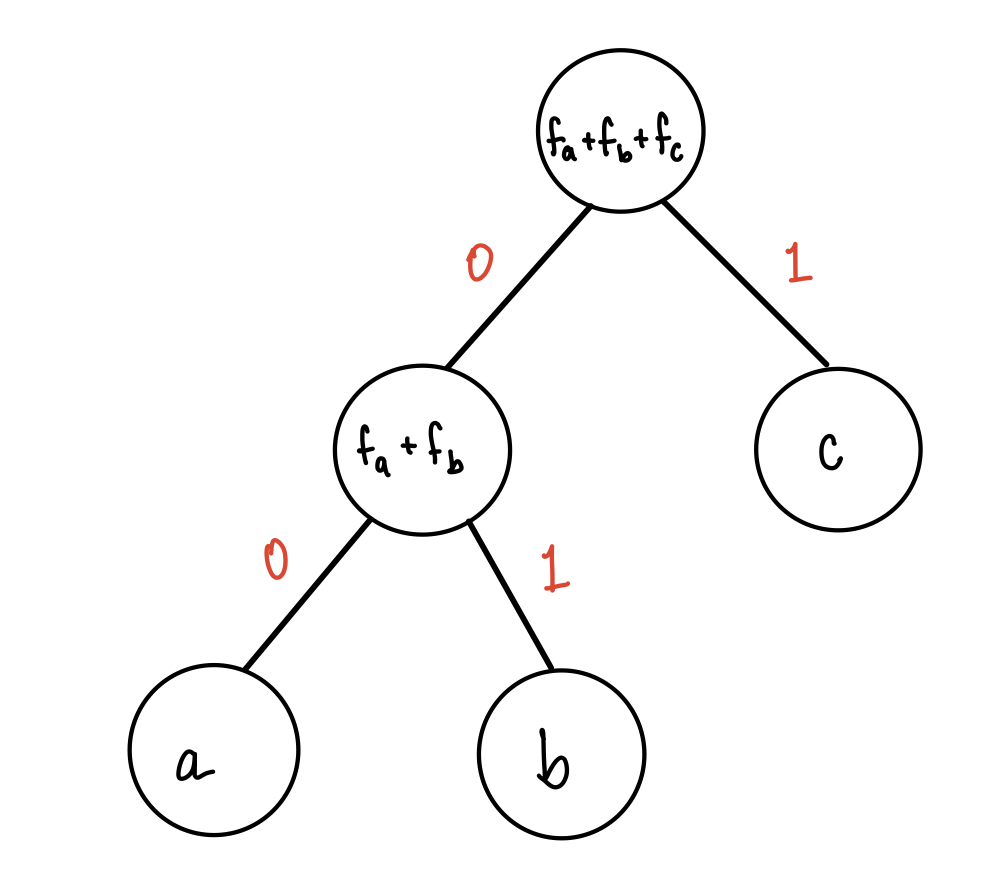
\includegraphics[scale=0.14]{answer6.png}\\
    $f_a < f_b < f_c$
    }
    
    \item{ (3 pts) For the given algorithm, solve the following.

You may assume the existence of a $\texttt{max}$ function taking $\mathcal{O}(1)$ time, which accepts at most four arguments and returns the highest of the four. \\
\begin{verbatim}
FindMax(A[0, ..., n-1]):
     if A.length == 1:
         return A[0]
    count = 0
    for i = 1 to n/2:
        count++
        
     return max( FindMax(A[0, ..., floor(n/4)], 
                 FindMax(A[floor(n/4) + 1, ..., floor(n/2)],
                 FindMax(A[floor(n/2) + 1, ..., floor(3n/4)],
                 FindMax(A[floor(3n/4) + 1, ..., n-1]))
\end{verbatim}
Find a recurrence for the worst-case runtime complexity of this algorithm. You can assume that $n$ is a multiple of four. Solve the recurrence found to obtain worst-case runtime complexity.
\makenonemptybox{6in}{
Recurrence relation for the following code:\\
Let $T(n)$ be the worst-case runtime where $T(n)= 4T(\frac{n}{4})+\mathcal{O}(n)+\mathcal{O}(1)$.\\
$= 4T(\frac{n}{4})+n$\\
\\
Using the master's method\\
$a=4$, $b=4$, $k=1$\\
$a=b^k$  $\rightarrow$  $4=4^1$\\
\\
Therefore we apply the second case of master theorem\\
$T(n)=\Theta(n^k\log n)$\\
The worst case runtime is $T(n)= \Theta(n\cdot \log n)$
}
}
    \clearpage
    \item{ (4 pts)
        Assume there are $n$ items $\{item_1, item_2, $ ... $item_n\}$, each item has a weight $w_i$ and value $v_i$ associated with it. You have a bag that can carry a maximum load of weight $W$. Each of the $n$ items can be divided into \textbf{fractions} such that the value and weight associated with the item decreases proportionally.\\
         The inputs to your function will be values $v$, weights $w$, number of items $n$ and capacity $W$.\\
        Provide well commented pseudo or actual code, that returns the maximum total value of all items that can be carried. \\
        Also briefly discuss the space and runtime complexity of your pseudo-code.\\
       
        \textbf{Input}\\
        $v$ = [20, 27, 18] \\
        $w$ = [2, 3, 3]\\
        $W = 3$  \\
        \textbf{Output}\\
        29 \\
        The Algorithm should pick $item_1$ and $\frac{1}{3}^{rd}$ of $item_2$ leading to a total value of $20 + 27 \frac{1}{3} = 29$.
    }
    \makenonemptybox{3in}{
    pseudo code on next page
    }
    \clearpage
    \makenonemptybox{6in}{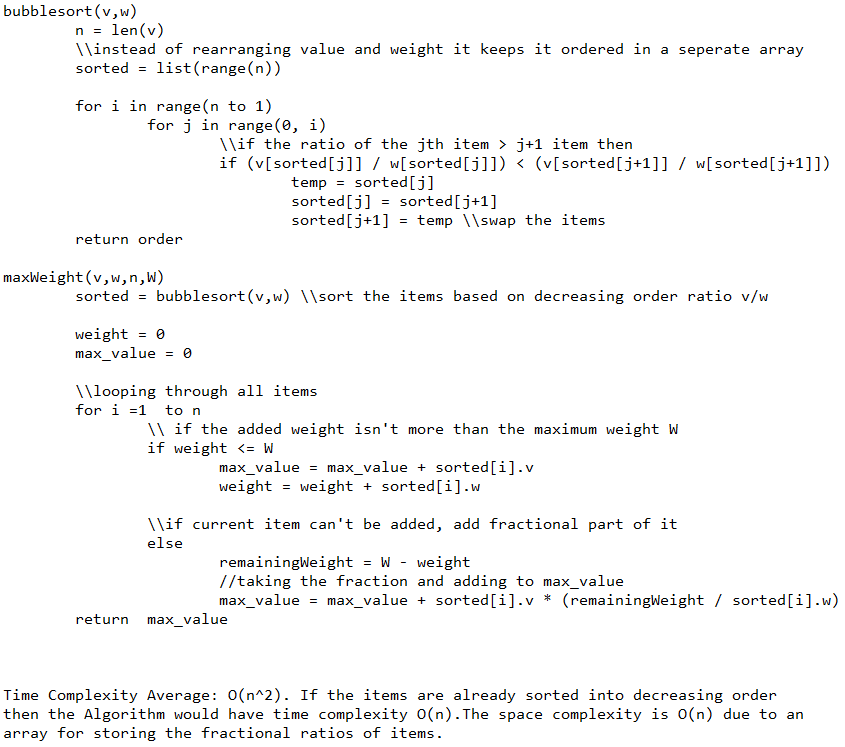
\includegraphics[scale=0.7]{answer8.png}}
    \clearpage
    \item{ (6 pts)
    Given an array $A$ and a value $k$, design a divide and conquer algorithm to find the $k^{th}$ smallest element in the array. The algorithm proposed should not use extra space i.e the space complexity of the algorithm should be constant $\Theta(1)$. Your algorithm must have an average case runtime of $\mathcal{O}(n\log(n))$. You can assume the access to a function which returns a random number within a range in constant time. You are allowed to modify the array passed as input.  \\
    The inputs to your function will be an array $A$ and value $k$.  \\
    Provide well commented pseudo or actual code for the algorithm. \\ \\
    Assume that you have access to a function \textit{rand(min, max)} which will return a random integer between \textit{min} and \textit{max} in constant time inclusive of both min and max.
    
    \textbf{Input}\\
        $A$ = [10, 13, 20, 8, 7, 6, 100] \\
        $k$ = 4\\
        \textbf{Output}\\
        10 \\ \\
        10 is the 4th smallest value in the given array.
    }
    \makenonemptybox{3in}{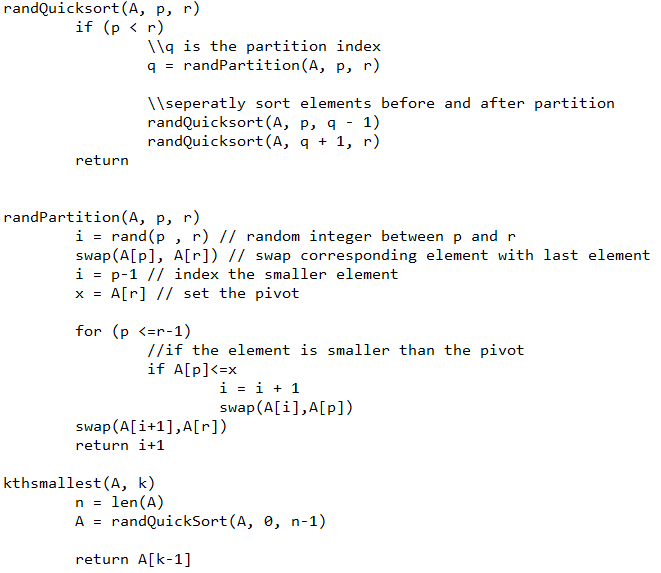
\includegraphics[scale=0.5]{answer9c.png}}
    \clearpage
    \item{(6 pts)
    Assume there are $n$ carrots and $n$ rabbits along a straight line.  
    Each rabbit needs to eat a carrot. Rabbits can move in either direction, simultaneously along the line and travelling 1 unit of distance takes 1 minute. Design a greedy algorithm that takes $\mathcal{O}(n\log(n))$ to assign carrots to rabbits such that the time taken to eat the last carrot is minimized. The algorithm should return the value of the time taken to eat last carrot.\\\
    You will be given the position of rabbits and carrots along the straight line.\\  \\
    \textbf{Expectations}
    \begin{itemize}
        \item  You should clearly describe the greedy choice that the algorithm makes in assigning carrots to rabbits.\\
        \item Provide well commented pseudo or actual code for the algorithm. \\
        \item Discuss the space and runtime complexity of the pseudo or actual code. 
    \end{itemize}
   
    
    \textbf{Example 1}: \\
    rabbits = [7, 3, 2, 13, 2] \\
    carrots = [1, 3, 5, 14, 21] \\
    output : 8 \\
    In this example the assignment is as follows.
    \begin{itemize}
        \item The carrot at distance 1 (index 0) is eaten by rabbit at distance 2 (index 4).
        \item  The carrot at distance 3 (index 1) is eaten by rabbit at distance 2 (index 2).
        \item The carrot at distance 5 (index 2) is eaten by rabbit at distance 3 (index 1).
        \item The carrot at distance 14 (index 3) is eaten by rabbit at distance 7 (index 0).
        \item The carrot at distance 21 (index 4) is eaten by rabbit at distance 13 (index 3), with 21-13=8 minutes being the longest time. 
        
    \end{itemize}
    
    \textbf{Example 2}: \\
    rabbits = [84, 15, 15, 161, 187, 9, 66, 1] \\ 
    carrots = [92, 103, 163, 119, 63, 117, 144, 172] \\
    output : 102
    }
    \makenonemptybox{7.5in}{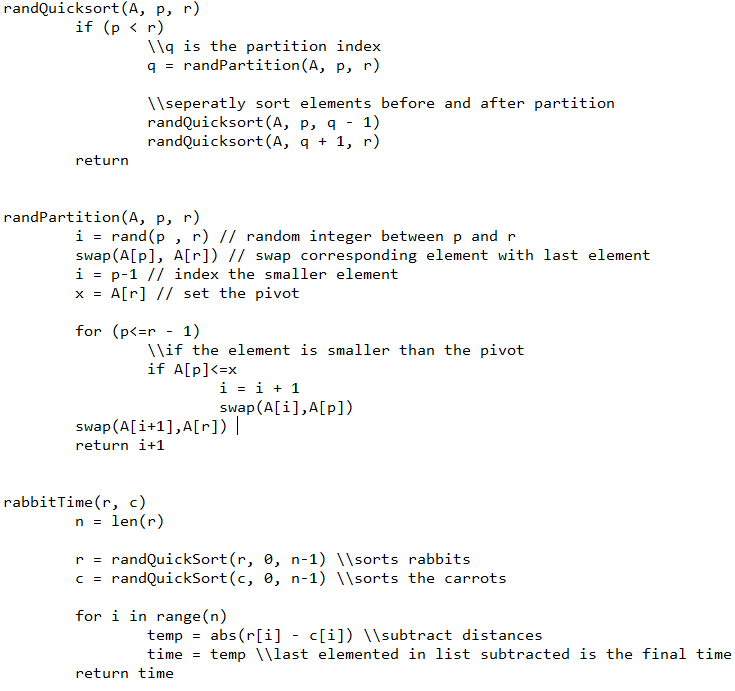
\includegraphics[scale=0.8]{answer10.png}}
    
    
    \item{\textbf{For extra credit pick one of the two questions provided. Extra credit will only be considered if your midterm score less than 100\% (2 pts)} \\ 
    

    Please provide your solution with proper comments, solutions without proper comments will not be considered.}
    
   \url{ https://leetcode.com/problems/gas-station/ }
   



\begin{center}
    \textbf{OR}
\end{center}   

 
  
    
   \url{  https://leetcode.com/problems/maximal-square/ }

    % Paste your code in the verbatim tag below

\begin{verbatim}
class Solution(object):
    def canCompleteCircuit(self, gas, cost):
        """TIME COMPLEXITY O(n)
            SPACE COMPLEXITY O(1)"""
        #we calculate the surpless and deficeit amounts to reach the station
        tank = currtank = start = 0 #starting 
        n = len(gas)
        for i in range(n):
            #refuel and drive to next station
            tank += gas[i] - cost[i]
            #if the sum the tank is a negative value
            if tank < 0:
                #set the value of tank to currtank
                currtank += tank
                """"print("tank1", currtank)"""
                #reset the value of tank
                tank = 0
                start = i + 1
        #currtank value is added to check if the refeul was enough
        currtank += tank
        """print(currtank, tank)"""
        #check to see if the currtank value is less than 0
        if currtank < 0: return -1
        #if we completed the full circle then return the the last value of start 
        else: return start
\end{verbatim}	
    
	
\end{enumerate}


\end{document}


